\documentclass[final,utf8]{beamer}
\mode<presentation>
{
  \usetheme{lspposter}
} 
\usepackage{amsmath,amssymb}
\usepackage{textcomp} 
\usepackage[orientation=portrait,size=a0,scale=1.4,debug]{beamerposter}
\usepackage{booktabs,array}
\usepackage{listings}
\usepackage{xspace}
\usepackage{fp}
\usepackage{ifthen} 
% \usepackage[utf8]{inputenc}
% \usepackage[T1]{fontenc}
 

% Display a grid to help align images
%\beamertemplategridbackground[1cm]

\title{\Huge Open-Access-Monographien und -Sammelb\"ande}

\author{Sebastian Nordhoff, FU Berlin}
\institute[Language Science Press]{Language Science Press} % (optional, but mostly needed)
% {Language Science Press}

\date{13.10.2014}

\begin{document}
\begin{frame}{} 
\vspace{-1cm}
\begin{columns}[t]
  %%%%%%%%%%%%%%%%%%%%%%%%%%%%%%%%%%%%%%%%%%%%%%%%%%%%%%%%%%%%%%%%%%%%%%%%%%%%%%%%%%%%%%%%%%%%%%%%%%%%
% 				      Erste Spalte
  %%%%%%%%%%%%%%%%%%%%%%%%%%%%%%%%%%%%%%%%%%%%%%%%%%%%%%%%%%%%%%%%%%%%%%%%%%%%%%%%%%%%%%%%%%%%%%%%%%%%
  \begin{column}{.45\linewidth}  
    \setbeamercolor*{block title}{bg=lsp1}
    \begin{block}{Language Science Press} 
	\begin{itemize}
	\item Monographien und Sammelb\"ande
	\item Sprachwissenschaft
	\item Open Access CC-BY
	\item Gratis PDF; Druck per Print-on-Demand m\"oglich (Hardcover/Softcover)
	\item ISBN, DOI, DOAB, OAPEN, GoogleBooks
	\item Anschubfinanzierung der DFG an der Freien Universit\"at 
	\item Jetzt grundst\"andig finanziert an der Humboldt-Universit\"at 
	\item Projektion: ab 2018 selbsttragend 
	\end{itemize} 
    \end{block}    

    \setbeamercolor*{block title}{bg=lsp2}
    \begin{block}{Community} 
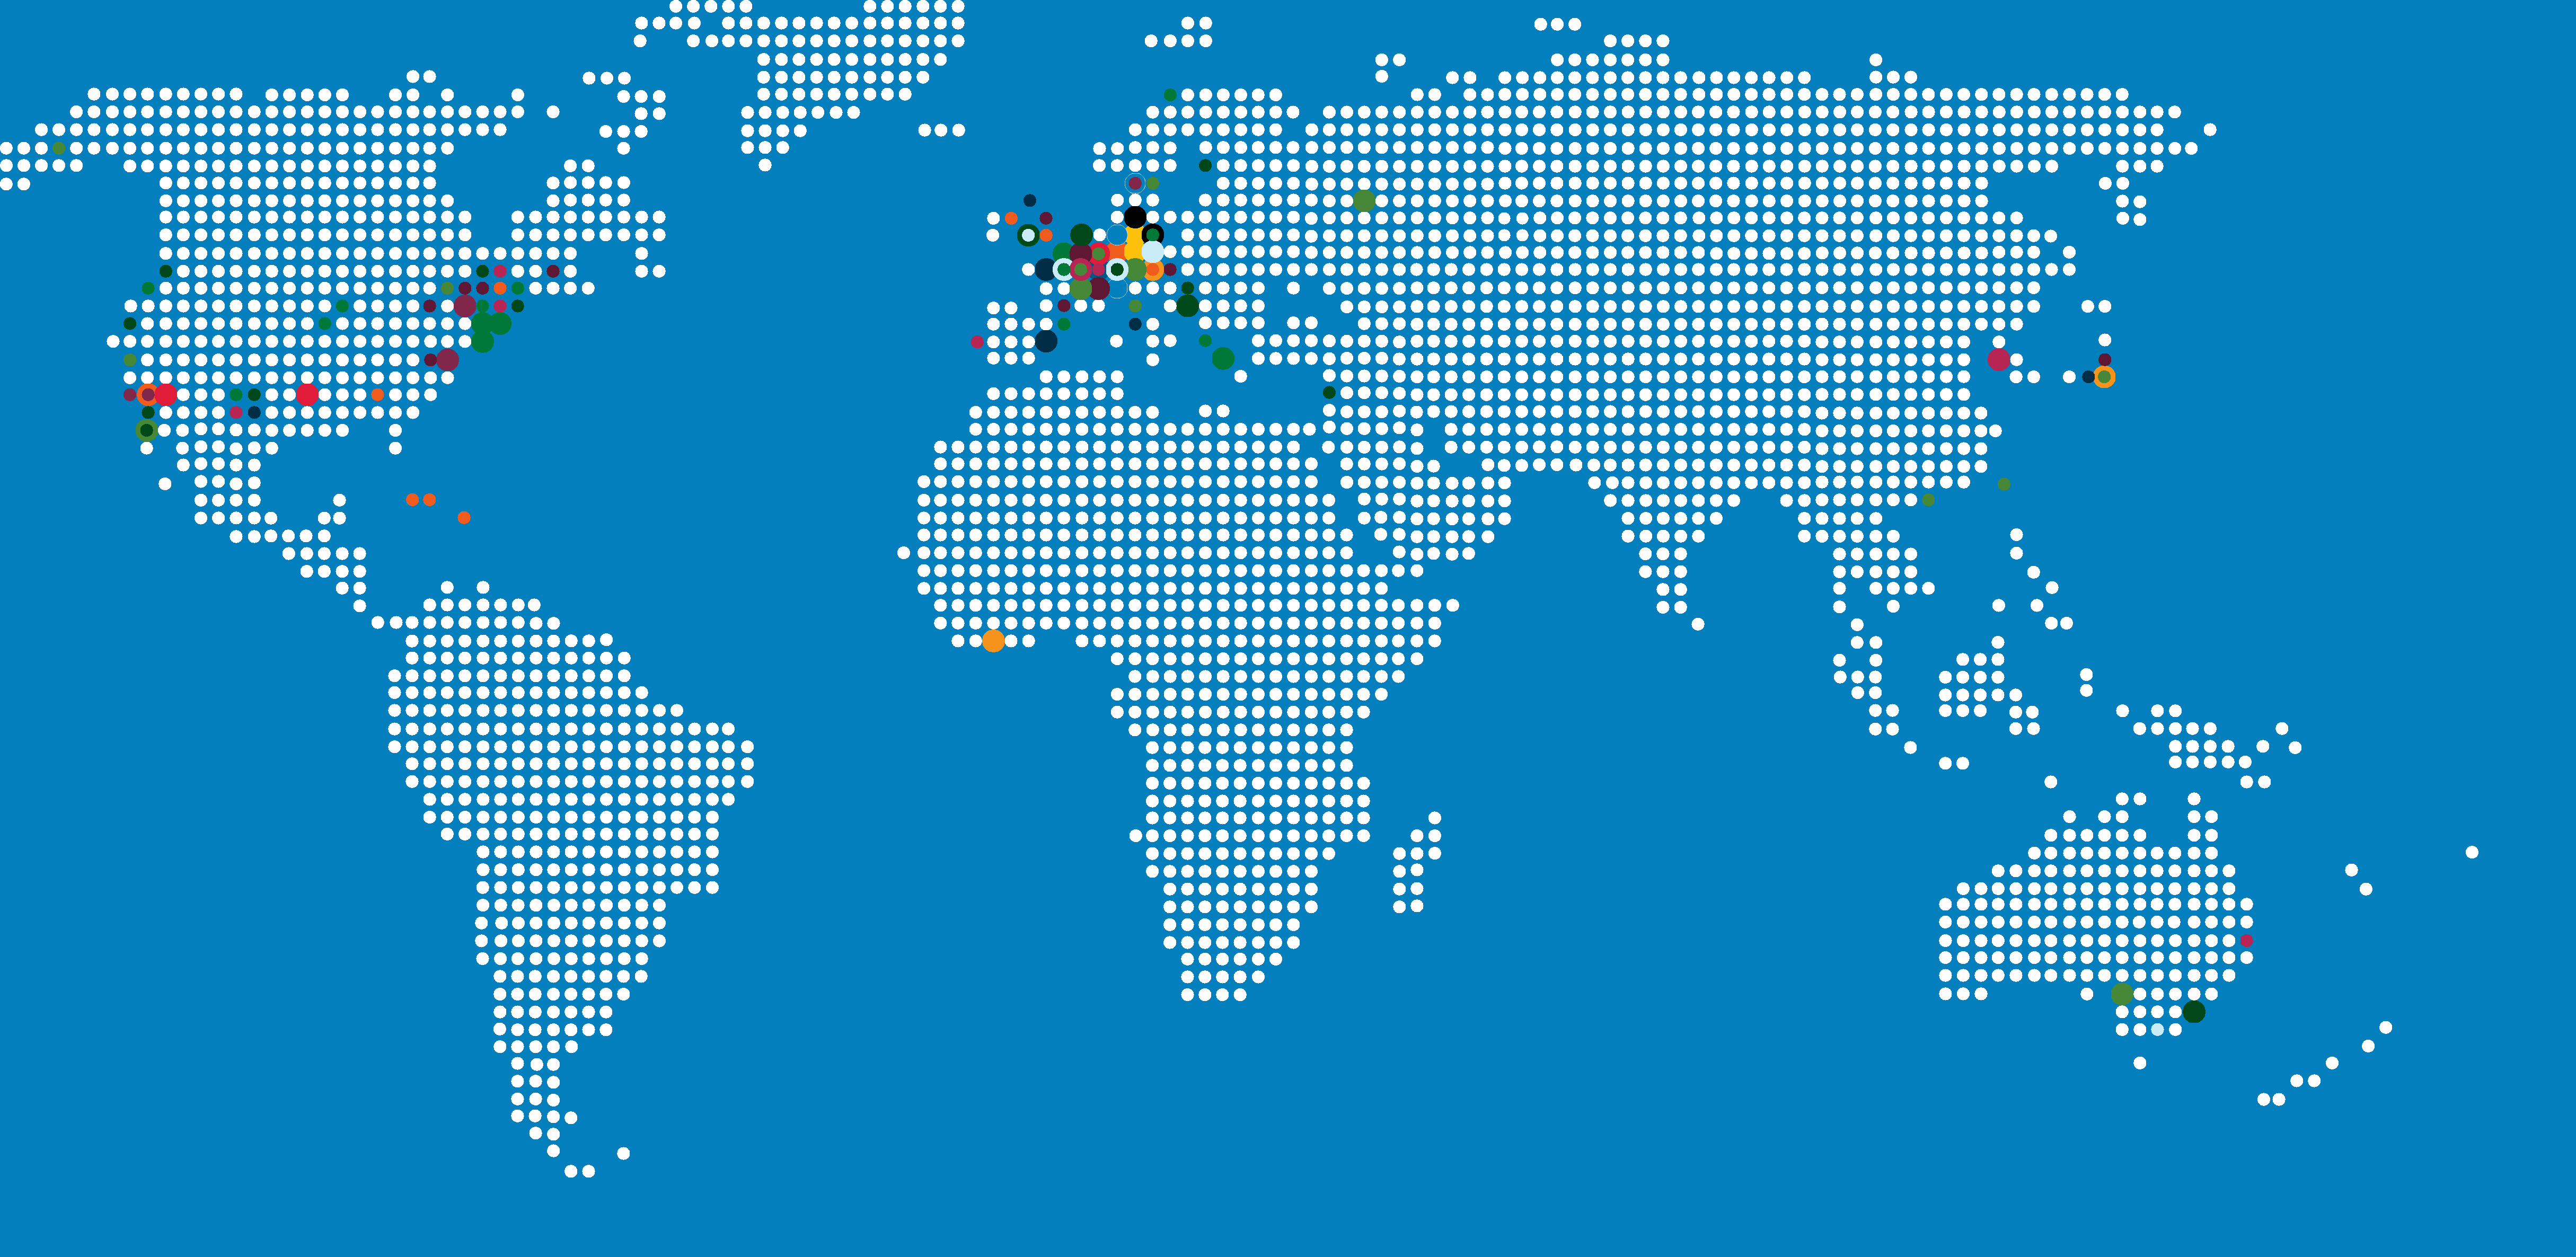
\includegraphics[width=.9\textwidth]{WORLDMAPDOTSdots.png}
	\begin{itemize} 
	    \item weltweite Autoren-, Leser- und Herausgeberschaft
	    \item weitl\"aufige Abdeckung der Subdisziplinen
	    \item 20 Reihen, 28 publizierte B\"ucher, 196 Anfragen (09/2016)
	    \item 623 Supporter, 194 Editorial Board Members, 165 Community Proofreader
	    \item \"uber 60.000 Downloads
	\end{itemize}  
    \end{block} 


    \setbeamercolor*{block title}{bg=lsp3}
    \begin{block}{Finanzierung} 
	\begin{enumerate} 
	    \item Printmarge
	    \item optionale Autorengeb\"uhren
	    \item institutionelle Mitgliedschaften \"uber Knowledge Unlatched
	    \item F\"ordermitglieder
	    \item Spenden
	\end{enumerate}  
    \end{block} 



    \setbeamercolor*{block title}{bg=lsp4}
    \begin{block}{Workflow} 
	\begin{enumerate} 
	    \item Webbasiert (Open Monograph Press) oder traditionell (Email)
	    \item Bucherstellung mit {\LaTeX}
	    \item MS Word$\to${\LaTeX}-Webkonverter
	    \item Manuskriptfinalisierung mit Overleaf
	\end{enumerate}  
     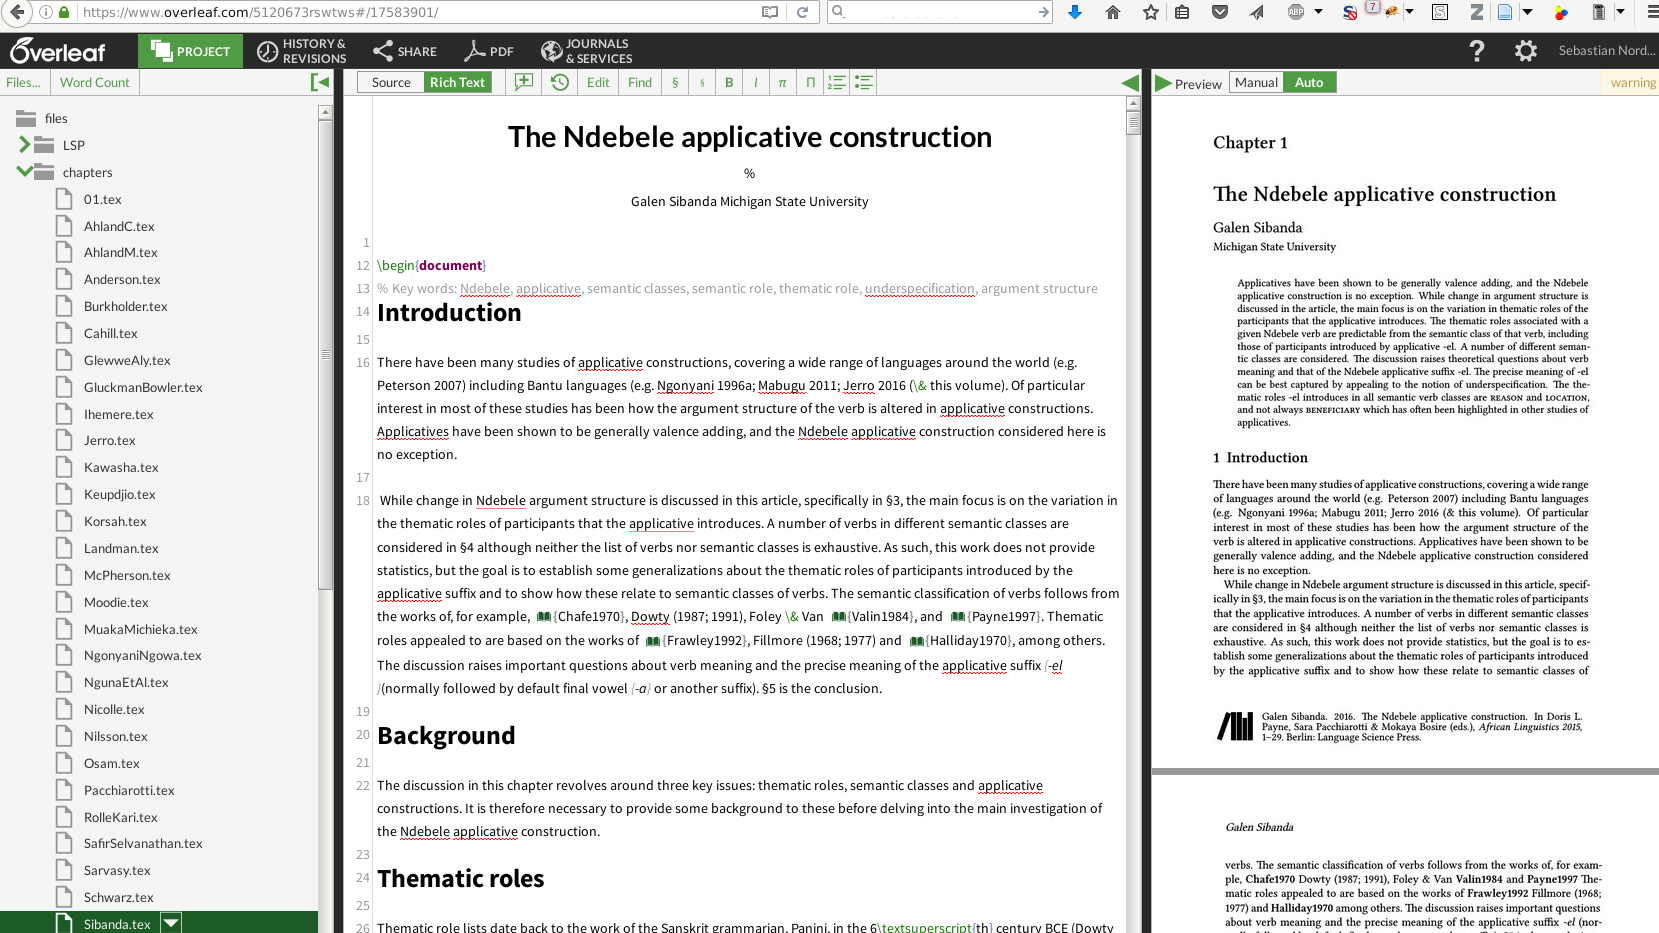
\includegraphics[width=.9\textwidth]{overleaf.png}
  
    \end{block} 

 

 

  \end{column}


  % bg=lsp2,3,4,5,6 etc f\"ur folgende K\"asten
  %%%%%%%%%%%%%%%%%%%%%%%%%%%%%%%%%%%%%%%%%%%%%%%%%%%%%%%%%%%%%%%%%%%%%%%%%%%%%%%%%%%%%%%%%%%%%%%%%%%%
% 				      Zweite Spalte
  %%%%%%%%%%%%%%%%%%%%%%%%%%%%%%%%%%%%%%%%%%%%%%%%%%%%%%%%%%%%%%%%%%%%%%%%%%%%%%%%%%%%%%%%%%%%%%%%%%%%
  \begin{column}{.45\linewidth}
    
    \setbeamercolor*{block title}{bg=lsp7}
    \begin{block}{Reihen}
      \begin{columns}
	\begin{column}{.48\textwidth}
	  \begin{itemize}
\item African Language Grammars and Dictionaries 
 \item Classics in Linguistics  
 \item Computational Models of Language Evolution  
 \item Conceptual Foundations of Language Science 
 \item Contemporary African Linguistics   
 \item Em­pir­i­cal­ly Ori­ent­ed The­o­ret­i­cal Mor­phol­o­gy and Syn­tax 
 \item Eurosla Studies
 \item Im­ple­ment­ed Gram­mars  
 \item Language Variation 
	  \end{itemize}
	\end{column}
	\begin{column}{.48\textwidth}
	  \begin{itemize}
 \item Monographs on Comparative Niger-Congo  
 \item Morphological Investigations 
 \item Multiword Expressions and Phraseology
 \item Open Generative Syntax  
 \item Studies in Diversity Linguistics  
 \item Studies in Laboratory Phonology  
 \item Textbooks in Language Sciences  
 \item Topics at the Grammar-Discourse Interface 
 \item Translation and Multilingual Natural Language Processing  
 \item Studies in Caribbean Languages  
	  \end{itemize}
      \end{column}
      \end{columns}
      \vskip1ex 
    \end{block}
    
    \setbeamercolor*{block title}{bg=lsp8}
    \begin{block}{B\"{u}cher}
      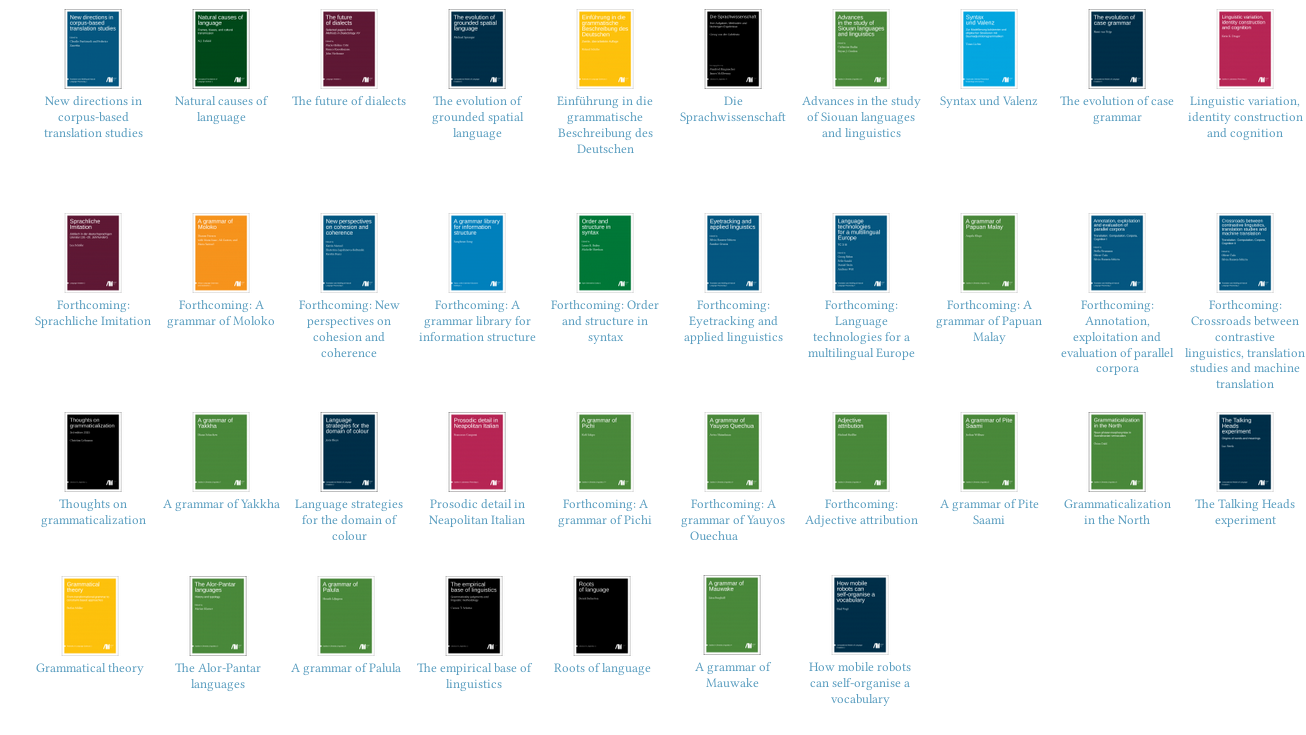
\includegraphics[width=.9\textwidth]{books.png}
    \end{block}  
  

    
    \setbeamercolor*{block title}{bg=lsp9}
    \begin{block}{Downloads}
      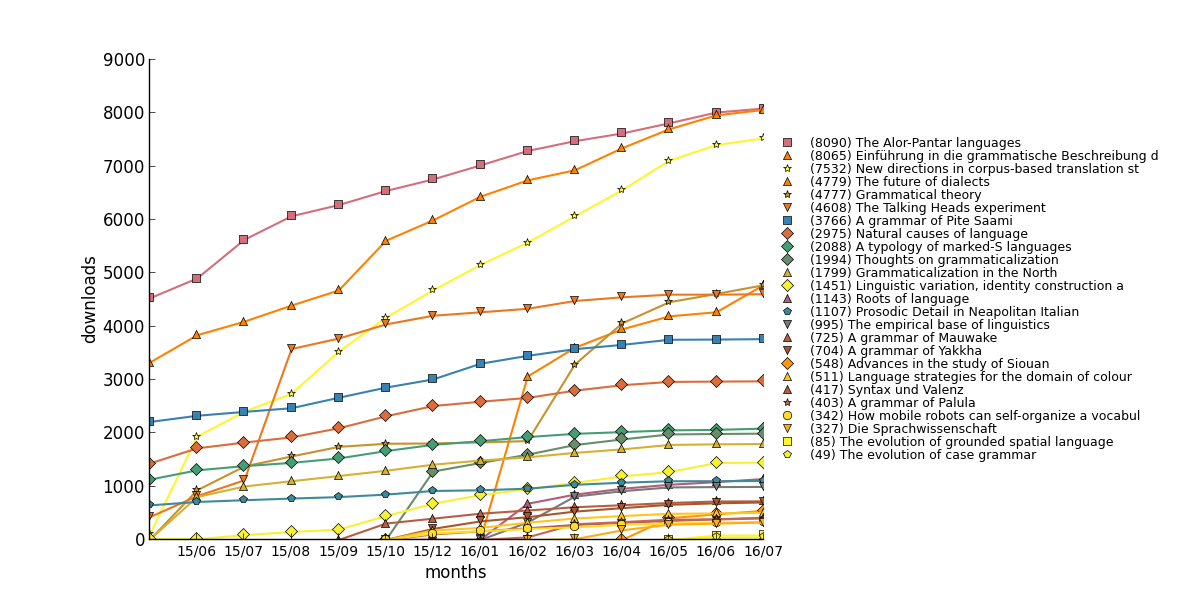
\includegraphics[width=.9\textwidth]{cumulativeall.png}
    \end{block}  
  

    \setbeamercolor*{block title}{bg=lsp10}
    \begin{block}{Unterst\"utzer werden}
     \raggedleft 
\includegraphics[width=.2\textwidth]{qrcode.png}
    \end{block}  
  


  \end{column}
  %%%%%%%%%%%%%%%%%%%%%%%%%%%%%%%%%%%%%%%%%%%%%%%%%%%%%%%%%%%%%%%%%%%%%%%%%%%%%%%%%%%%%%%%%%%%%%%%%%%%
  %%%%%%%%%%%%%%%%%%%%%%%%%%%%%%%%%%%%%%%%%%%%%%%%%%%%%%%%%%%%%%%%%%%%%%%%%%%%%%%%%%%%%%%%%%%%%%%%%%%%
\end{columns}
\vfill
\end{frame}

\end{document}


%%%%%%%%%%%%%%%%%%%%%%%%%%%%%%%%%%%%%%%%%%%%%%%%%%%%%%%%%%%%%%%%%%%%%%%%%%%%%%%%%%%%%%%%%%%%%%%%%%%%
%%% Local Variables: 
%%% mode: latex
%%% TeX-PDF-mode: t